\documentclass[tikz]{standalone}
\usepackage[utf8]{inputenc}
\usetikzlibrary{calc}

\def\rayon{2}
\def\anglestart{120}

\begin{document}

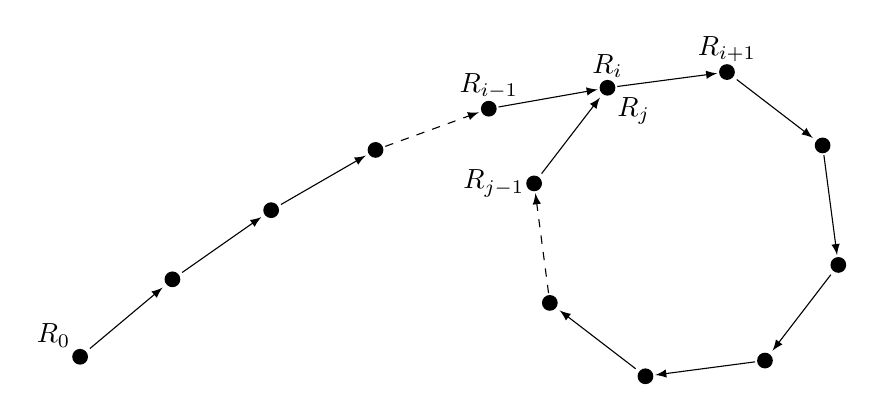
\begin{tikzpicture}

\node (R0) at (0,0) {};
\path (R0) arc (\anglestart:\anglestart-45:\rayon) node (R1) {}
           arc (\anglestart-45:\anglestart-90:\rayon) node (R2) {}
           arc (\anglestart-90:\anglestart-135:\rayon) node (R3) {}
           arc (\anglestart-135:\anglestart-180:\rayon) node (R4) {}
           arc (\anglestart-180:\anglestart-225:\rayon) node (R5) {}
           arc (\anglestart-225:\anglestart-270:\rayon) node (R6) {}
           arc (\anglestart-270:\anglestart-315:\rayon) node (R7) {};
        
\path let \p1 = ($(R0) - (R1)$)
      in (R0) --++ (190:{veclen(\x1,\y1)}) node (S4) {}
      --++ (200:{veclen(\x1,\y1)}) node (S3) {}
      --++ (210:{veclen(\x1,\y1)}) node (S2) {}
      --++ (215:{veclen(\x1,\y1)}) node (S1) {}
      --++ (220:{veclen(\x1,\y1)}) node (S0) {};

\fill (R0) circle (.1);
\fill (R1) circle (.1);
\fill (R2) circle (.1);
\fill (R3) circle (.1);
\fill (R4) circle (.1);
\fill (R5) circle (.1);
\fill (R6) circle (.1);
\fill (R7) circle (.1);

\fill (S0) circle (.1);
\fill (S1) circle (.1);
\fill (S2) circle (.1);
\fill (S3) circle (.1);
\fill (S4) circle (.1);

\draw[-latex] (R0) -- (R1);
\draw[-latex] (R1) -- (R2);
\draw[-latex] (R2) -- (R3);
\draw[-latex] (R3) -- (R4);
\draw[-latex] (R4) -- (R5);
\draw[-latex] (R5) -- (R6);
\draw[-latex,dashed] (R6) -- (R7);
\draw[-latex] (R7) -- (R0);

\draw[-latex] (S0) -- (S1);
\draw[-latex] (S1) -- (S2);
\draw[-latex] (S2) -- (S3);
\draw[-latex,dashed] (S3) -- (S4);
\draw[-latex] (S4) -- (R0);

\node[above left] at (S0) {$R_0$};
\node[above] at (R0) {$R_i$};
\node[below right] at (R0) {$R_j$};
\node[left] at (R7) {$R_{j-1}$};
\node[above] at (S4) {$R_{i-1}$};
\node[above] at (R1) {$R_{i+1}$};

\end{tikzpicture}

\end{document}